\documentclass[nobib]{tufte-handout}

\title{Föreläsning 8: Träd och heltalspartitioner $\cdot$ 1MA020}

\author[Vilhelm Agdur]{Vilhelm Agdur\thanks{\href{mailto:vilhelm.agdur@math.uu.se}{\nolinkurl{vilhelm.agdur@math.uu.se}}}}

%\date{7 februari 2023}


%\geometry{showframe} % display margins for debugging page layout

\usepackage{graphicx} % allow embedded images
  \setkeys{Gin}{width=\linewidth,totalheight=\textheight,keepaspectratio}
  \graphicspath{{graphics/}} % set of paths to search for images
\usepackage{amsmath}  % extended mathematics
\usepackage{booktabs} % book-quality tables
\usepackage{units}    % non-stacked fractions and better unit spacing
\usepackage{multicol} % multiple column layout facilities
\usepackage{lipsum}   % filler text
\usepackage{fancyvrb} % extended verbatim environments
  \fvset{fontsize=\normalsize}% default font size for fancy-verbatim environments

\usepackage{color,soul} % Highlights for text

% Standardize command font styles and environments
\newcommand{\doccmd}[1]{\texttt{\textbackslash#1}}% command name -- adds backslash automatically
\newcommand{\docopt}[1]{\ensuremath{\langle}\textrm{\textit{#1}}\ensuremath{\rangle}}% optional command argument
\newcommand{\docarg}[1]{\textrm{\textit{#1}}}% (required) command argument
\newcommand{\docenv}[1]{\textsf{#1}}% environment name
\newcommand{\docpkg}[1]{\texttt{#1}}% package name
\newcommand{\doccls}[1]{\texttt{#1}}% document class name
\newcommand{\docclsopt}[1]{\texttt{#1}}% document class option name
\newenvironment{docspec}{\begin{quote}\noindent}{\end{quote}}% command specification environment

\include{mathcommands.extratex}

\begin{document}

\definecolor{darkgreen}{rgb}{0.0627, 0.4588, 0.1451}

\maketitle% this prints the handout title, author, and date

\begin{abstract}
\noindent
Vi introducerar grafer och träd, och bevisar att antalet rotade ordnade binära oetiketterade träd också räknas av Catalantalen.

Sedan introducerar vi heltalspartitioner, och härleder en genererande funktion för dessa, som vi använder för några exempel.
\end{abstract}

\section{Grafer och träd}

Vårt första ämne i denna föreläsning är grafer och träd, som kommer dyka upp igen och igen också i senare föreläsningar -- det är ju till och med den preliminära titeln på vår sista föreläsning. Vi börjar med att ge en samling definitioner av vad vi menar med dessa ord, och sedan börjar vi räkna hur många av olika typer av graf det finns i olika klasser.

\begin{definition}
    En \emph{graf} består av en mängd $V$ av \emph{noder} och en mängd $E \subseteq \binom{V}{2}$ av kanter.\sidenote[][]{Med notationen $\binom{A}{k}$ där $A$ är en mängd och $k$ ett heltal menar vi \emph{mängden} av delmängder av storlek $k$ till $n$. Alltså har vi att
    $$\abs{\binom{[n]}{k}} = \binom{n}{k}.$$} Om det finns en kant $\{u,v\}$ säger vi att $u$ och $v$ är \emph{grannar}. En graf är \emph{etiketterad} om noderna är särskiljbara, annars är den oetiketterad.
    \sidenote[][]{Det här är precis samma koncept som med våra lådor som var särskiljbara eller inte. Antingen har noderna namn, så vi kan prata om nod nummer tre, eller så kan vi bara se vilka andra noder de har kanter till.} 
    Vi säger att en graf är \emph{sammanhängande} om det går att nå varje nod från varje annan nod genom att vandra längs kanterna. Ett sätt att vandra från en nod tillbaka till sig själv kallar vi för en \emph{cykel}.

    \begin{figure}
        \centering
        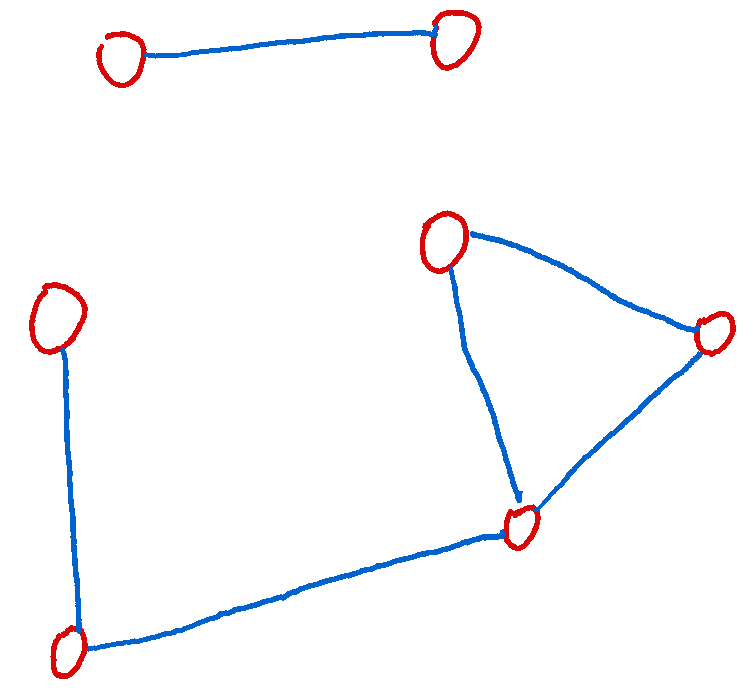
\includegraphics[width=0.4\textwidth]{graphics/example_graph.png}
        \caption[][2cm]{Ett exempel på en graf. Den är inte sammanhängande, eftersom de övre två noderna inte kan nås från de undre fem. Triangeln utgör en cykel, som är grafens enda.}
    \end{figure}
\end{definition}

\begin{example}
    Det finns $2^{\binom{n}{2}}$ stycken etiketterade grafer på $n$ noder, eftersom det finns $\binom{n}{2}$ möjliga kanter, och vi får en graf per val av vilka kanter som skall vara med.

    Problemet med att räkna antalet oetiketterade grafer på $n$ noder är betydligt mer komplicerat. Den första idén man hade haft är kanske att det borde vara
    $$\frac{2^{\binom{n}{2}}}{n!}$$
    eftersom det borde finnas $n!$ olika sätt att sätta dit etiketterna. Problemet är att vissa grafer har symmetrier som gör att till synes olika sätt att skriva dit etiketter i själva verket ger samma etiketterade graf.

    \begin{figure}
        \centering
        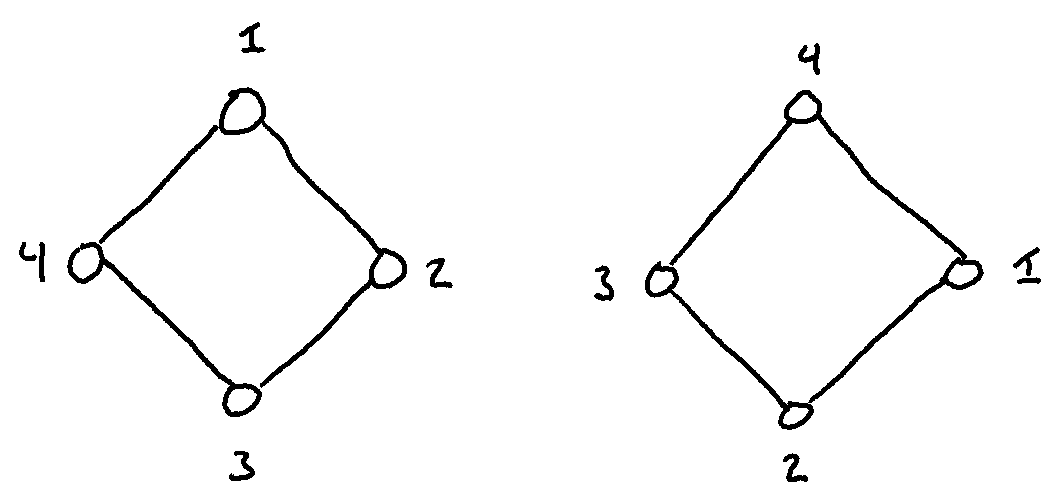
\includegraphics[width=0.5\textwidth]{graphics/counting_labelled_graphs.png}
        \caption{Två till synes olika etiketteringar av samma graf, som i själva verket är samma etikettering på grund av grafens rotationssymmetri.}
    \end{figure}

    Som tur är visar det sig att nästan alla grafer inte har någon symmetri alls, så svaret är \emph{nästan} $\frac{2^{\binom{n}{2}}}{n!}$.\sidenote[][-1.5cm]{Det här påståendet låter kanske löst i kanten, men det är faktiskt helt rigoröst. I alla fall om man ersätter ``nästan'' med att skriva att antalet är
    $$(1 + o(1))\frac{2^{\binom{n}{2}}}{n!}.$$}
\end{example}

\begin{definition}
    \begin{marginfigure}
        \centering
        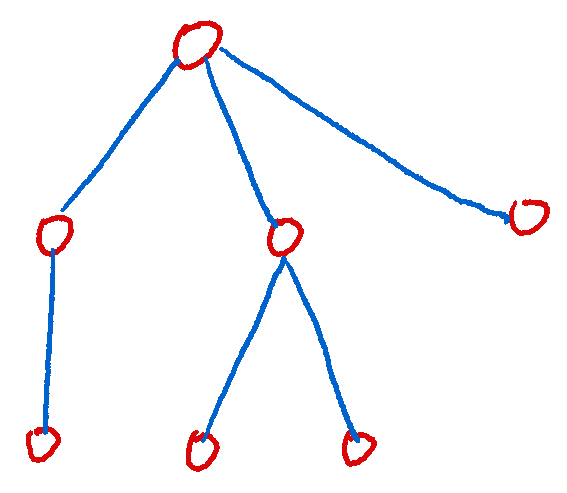
\includegraphics[width=0.6\textwidth]{graphics/example_tree.png}
        \caption{Ett träd med sju noder och sex kanter.}
    \end{marginfigure}

    Ett \emph{träd} är en sammanhängande graf utan cykler. Ett \emph{rotat} träd är ett träd med en specifik nod utpekad som dess rot.\sidenote[][]{Så om trädet är oetiketterat kan vi alltså se vilken nod som är roten, men resten av noderna kan vi inte se skillnad på, bara vilka som hänger ihop med vilka med kanter.} I ett rotat träd har varje nod utom roten själv en granne som är närmre roten än sig\sidenote[][]{Eller är roten.}, vilken vi kallar dess \emph{förälder}. Alla dess andra grannar kallar vi dess \emph{barn}. En nod utan barn kallar vi för ett \emph{löv}, och en nod som inte är ett löv kallar vi för \emph{intern}.

    Ifall det spelar roll i vilken ordning vi ritat noderna kallar vi trädet \emph{ordnat}, se figur \ref{fig:distinct_only_as_ordered}.

    \begin{marginfigure}
        \centering
        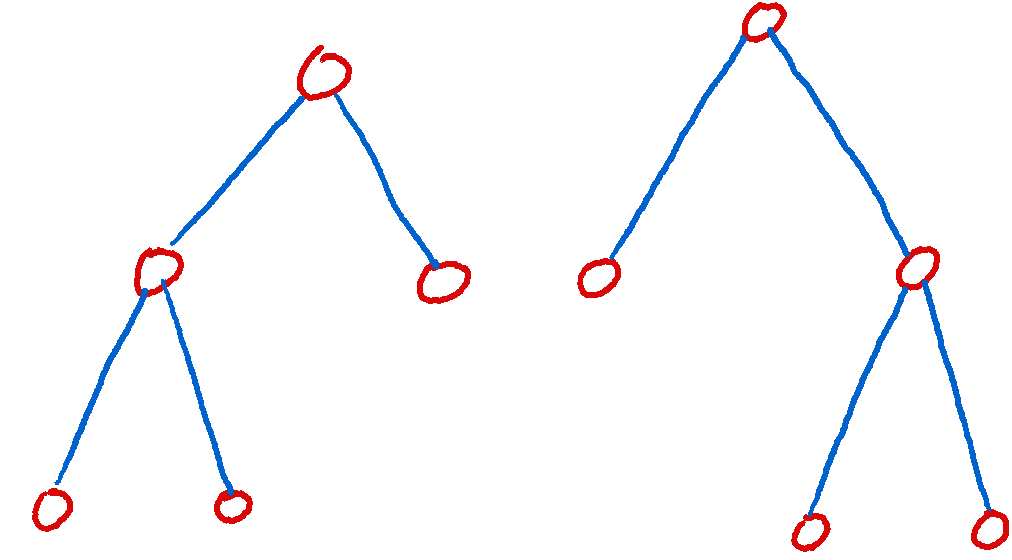
\includegraphics[width=0.8\textwidth]{graphics/ordered_versus_unordered_trees.png}
        \caption{Två träd som är olika varandra som ordnade träd, men samma träd som oordnade träd.}
        \label{fig:distinct_only_as_ordered}
    \end{marginfigure}
\end{definition}

\begin{definition}
    Ett träd i vilket alla noder antingen har två eller noll barn kallas för ett \emph{binärt} träd.
\end{definition}

Låt oss nu återse en gammal vän, Catalantalen.

\begin{proposition}
    Antalet rotade ordnade binära oetiketterade träd med $n$ stycken interna noder ges av Catalantalen.

    \begin{proof}
        Vi kan dela upp ett sådant träd i två mindre träd genom att helt enkelt ta bort roten, och låta dess två barn vara rötter i två mindre träd.

        \begin{figure}
            \centering
            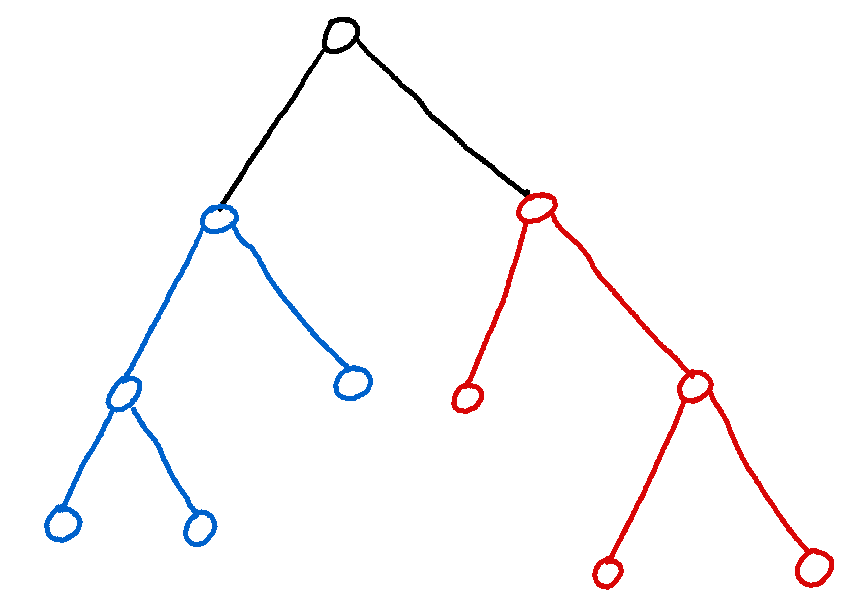
\includegraphics[width=0.5\textwidth]{graphics/RUBOTree_division.png}
            \caption[][1.5cm]{Ett rotat ordnat binärt oetiketterat träd, med uppdelningen av det i två mindre träd av samma typ, ett rött och ett blått.}
        \end{figure}

        Alltså gäller det, om $t_n$ betecknar antalet sådana träd, att
        $$t_{n+1} = \sum_{k=0}^{n} t_k t_{n-k},$$
        eftersom vi kan skapa oss ett sådant träd med $n+1$ noder genom att först rita roten, och sedan fästa ett träd med $k$ interna noder till vänster och ett med $n-k$ interna noder till höger. Eftersom roten själv är intern har vi då $k + n - k + 1 = n + 1$ interna noder.
    \end{proof}
\end{proposition}

\section{Cayleys formel}

Vi har alltså lyckats räkna en väldigt specifik sorts träd. Kan vi räkna träd mer generellt?

\begin{theorem}
    Det finns
    $$n^{n-2}$$
    stycken etiketterade träd med $n$ noder.
\end{theorem}

För att förstå detta resultat, låt oss börja med att räkna de första små fallen. Vi kollar på \emph{oetiketterade} träd, och räknar hur många sätt vi kan sätta etiketter på dem.

\begin{figure}
    \centering
    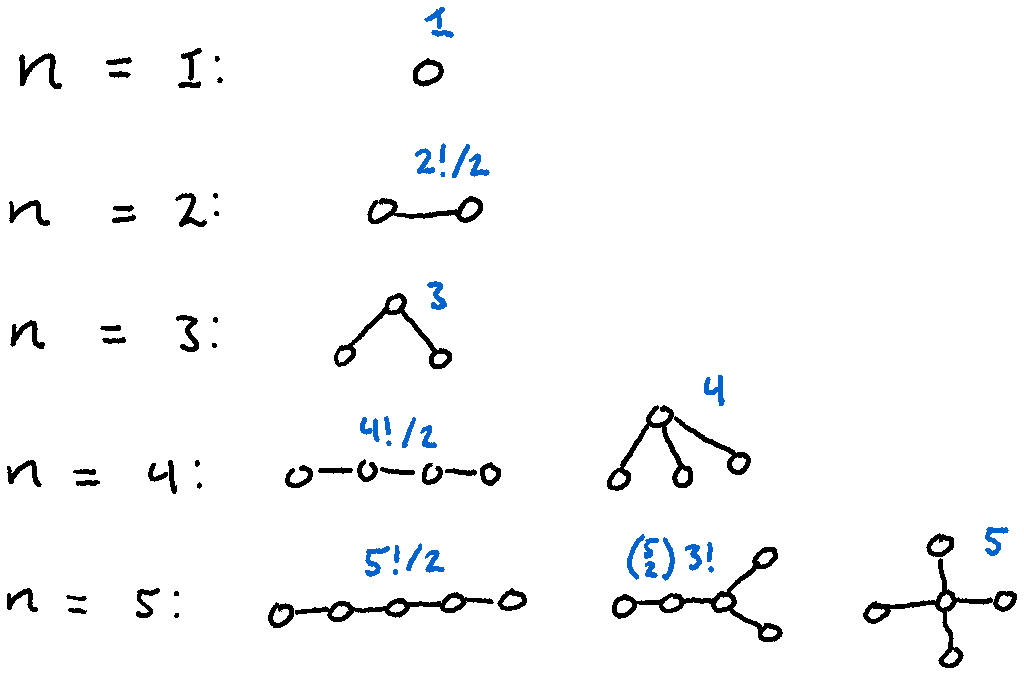
\includegraphics[width = \textwidth]{graphics/counting_tree_labellings.png}
    \caption{Oetiketterade grafer med $n$ noder, för $n = 1,\ldots,5$, med antalet sätt att sätta etiketter på varje i blått.}
\end{figure}

Sätten vi får dessa antal är, per värde på $n$:
\begin{enumerate}
    \item Att det bara finns ett sätt att skriva en etta på den enda noden är uppenbart.
    \item Vi kan välja vilken permutation som helst av $[2]$ att skriva på noderna, men grafen har en speglingssymmetri, så att skriva etiketterna i motsatt ordning ger samma träd. Alltså $\frac{2!}{2}$.
    \item Vi kan se vilken nod som är den mellersta, men vi kan inte se skillnad på de två yttre. Alltså är det enda val vi kan göra det av vilket tal vi skriver på den mellersta, vilket vi kan välja på tre sätt.
    \item För den första av våra två oetiketterade grafer kan vi skriva vilken permutation av $[4]$ vi vill, men återigen har vi en speglingssymmetri, så att skriva den baklänges ger oss samma etikettering. Alltså $\frac{4!}{2}$.
    
    För den andra är vi i samma situation som vi var i för $n=3$ -- vi kan se vilken nod det är som har mer än en granne, men vi kan inte se skillnad på de andra. Alltså är det enda valet vi har vilken etikett just den särskilda noden får, vilket vi kan göra på $4$ sätt.
    \item Vi får $\frac{5!}{2}$ av samma speglingssymmetri-skäl som innan, och för den tredje av våra grafer får vi $5$ eftersom vi åter har en särskild nod och resten kan vi inte se skillnad på.
    
    För den mellersta av våra tre oetiketterade träd kan vi se skillnad på de tre noderna i svansen till vänster, men de två som sticker ut åt höger kan vi inte se skillnad på. Så för att etikettera denna väljer vi två etiketter för de talen, vilket vi kan göra på $\binom{5}{2}$ sätt, och sedan är varje permutation av de återstående tre etiketterna faktiskt en distinkt etikettering, så vi kan välja $3!$ sätt att fullfölja vår etikettering. Så vi har totalt $\binom{5}{2}3!$ sätt att göra detta på.
\end{enumerate}

Så vi ser i alla fall att vår formel gäller för $n$ upp till fem. Vi väljer att ge två bevis för denna sats. Det första är av Prüfer, och ger en bijektion mellan etiketterade träd och en enklare mängd.

\begin{proof}[Prüfers bevis av Cayleys formel (1918)]
    Vi vill visa på en bijektion mellan mängden av etiketterade träd på $n$ noder och mängden av ord av längd $n-2$ ur alfabetet $[n]$. Att den senare mängden har rätt antal element vet vi sedan innan, så om vi kan hitta en bijektion är vi klara.

    Vi börjar med att berätta hur vi skapar vårt ord givet ett etiketterat träd.\sidenote[][-0.5cm]{Detta ord kallas för trädets \emph{Prüferkod}.} Vi letar upp det löv\sidenote[][]{Strikt sett har vi hittills bara definierat \emph{löv} för rotade träd -- och de träd vi studerar här har ju ingen rot-nod. Med ``löv'' menar vi här ``nod med bara en granne''.} som har lägst etikett, skriver dess etikett som första bokstav i vårt ord, och tar sedan bort noden ur trädet.

    \begin{figure}
        \centering
        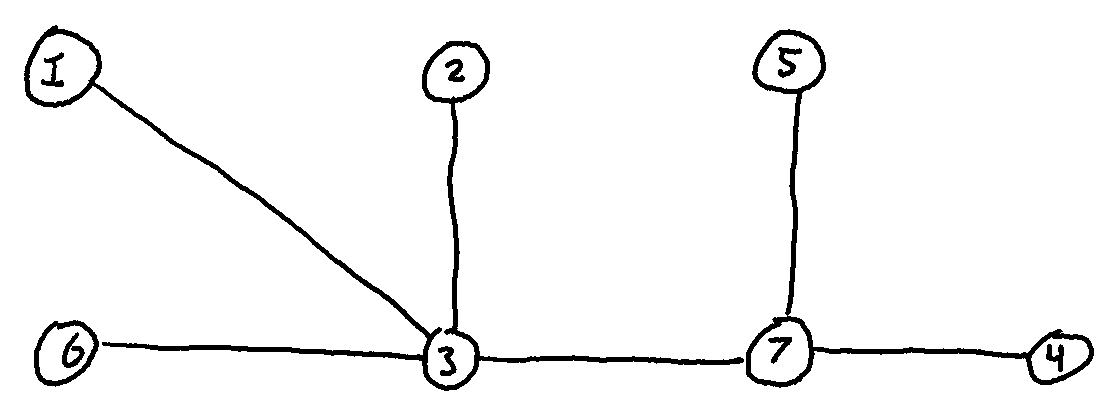
\includegraphics[width=0.75\textwidth]{graphics/prufer_code_tree_example.png}
        \caption[][1.25cm]{Ett etiketterat träd med Prüferkod $33773$.}
    \end{figure}

    Vi upprepar denna process -- letar upp det löv i det resulterande trädet som har lägst etikett (och notera att vi, när vi tar bort ett löv, ibland kommer göra en nod som innan var intern till ett löv), skriver den etiketten på slutet av ordet, och tar bort lövet. Processen fortsätter tills vi bara har två noder kvar.

    För att gå från en Prüferkod till en etiketterad graf använder vi följande algoritm, som konstruerar ett etiketterat träd givet en Prüferkod $a_1a_2\ldots a_{n-2}$.

    \begin{algorithm}
        \caption{Konstruktion av träd från Prüferkoder}\label{alg:constr_tree_from_prufer_code}
        \begin{algorithmic}
            \State Låt $G$ vara en graf med $n$ noder, med etiketter $1, 2, \ldots, n$, men utan kanter
            \State $L_1 \gets (1, 2, \ldots, n)$
            \State $A_1 \gets (a_1, a_2, \ldots, a_{n-2})$
            \For{$t = 1, 2, \ldots$}
            \If{$\abs{L_t} = 2$}
            \State Rita en kant i $G$ mellan de två elementen i $L$
            \State \textbf{stop}
            \Else
            \State Låt $l$ vara det minsta elementet i $L_t$ som inte är i $A_t$
            \State Låt $a$ vara det första elementet i $A_t$
            \State Rita en kant i $G$ mellan $l$ och $a$
            \State $L_{t+1} \gets L_t \setminus \{l\}$
            \State $A_{t+1} \gets (A_t(2), A_t(3), \ldots, A_t(\abs{A_t}))$
            \EndIf
            \EndFor\\
            \Return $G$
        \end{algorithmic}
    \end{algorithm}

    Det tar en stund att förstå vad den här algoritmen faktiskt gör\sidenote[][]{En fördel med föreläsningar över text är att man faktiskt kan genomföra algoritmen på ett konkret exempel, för att illustrera den, men en text måste så klart vara statisk. Sitter du hemma och läser föreslår jag att du prövar att göra algoritmen för hand på någon eller några Prüferkoder, för att få en känsla för vad som pågår.}, men efter en stunds kontemplation ser man att vad den gör är att den lägger till kanterna i precis den ordning som de försvann när vi skapade Prüferkoden.

    \begin{figure}
        \centering
        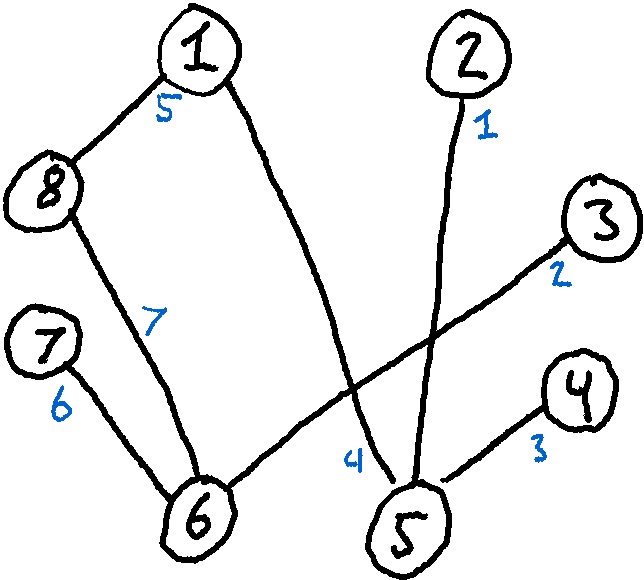
\includegraphics[width=0.6\textwidth]{graphics/tree_from_prufer_code.png}
        \caption{Ett träd skapat från Prüferkoden $565186$. I blått har vi markerat i vilket steg i algoritmen varje kant lades till -- lägg märke till att detta är precis ordningen i vilken de \emph{tas bort} om vi skapar Prüferkoden för detta trädet.} 
    \end{figure}

    Den första kanten att ritas kommer gå mellan det första lövet att tas bort och dess granne, den andra går mellan andra lövet att tas bort och dess granne, och så vidare -- ända fram tills den sista kanten vi lägger till, som går mellan de två kvarvarande noderna när vi byggde Prüferkoden. Alltså kommer denna algoritmen precis att rekonstruera grafen vi började med, vilket bevisar att vi faktiskt har en bijektion, och satsen följer.
\end{proof}

\section{Övningar}

\begin{xca}
    Bevisa att ett träd alltid har $\abs{E} = \abs{V} - 1$.
\end{xca}

\begin{xca}
    Överväg följande skiss av ett oetiketterat träd med $1 + i + j + k$ noder:
    \begin{figure}
        \centering
        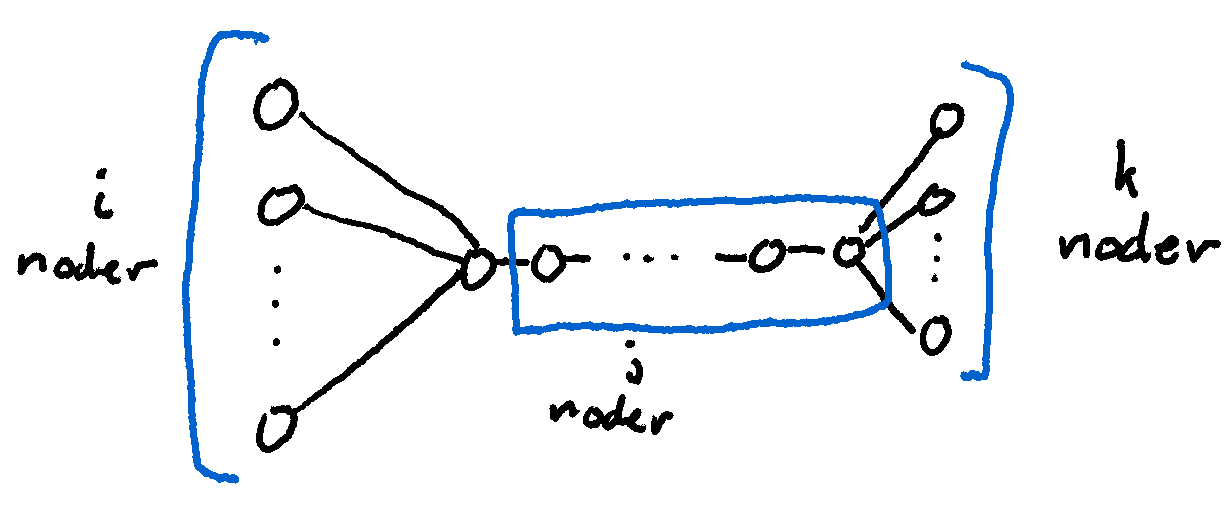
\includegraphics[width=0.8\textwidth]{graphics/exercise_label_unlabelled_tree.png}
        \caption{Skiss av ett oetiketterat träd.}
    \end{figure}

    Hur många olika sätt finns det att sätta etiketter på detta träd?\sidenote[][]{Vi resonerade om detta för några små träd precis efter att vi introducerade Cayleys formel, men här har vi alltså ett mer generellt fall.} Ge en formel som gäller för alla $i, j, k = 0, 1, 2,\ldots$.\sidenote[][]{Finns det några specialfall för särskilda kombinationer av värden på $i$, $j$, och $k$?}
\end{xca}

\begin{xca}
    Rita det etiketterade trädet som har Prüferkod $1273262$.
\end{xca}

\begin{xca}
    \emph{En övning för dig som kan programmera.}\sidenote[][]{För inlämningsuppgiften i kursen är denna uppgift frivillig om ni inte har någon i er grupp som kan programmering. Om ni genomför den, vänligen använd inte Matlab, eftersom jag inte kan köra sådan kod. Mathematica är okej.} Implementera vår algoritm för att omvandla en Prüferkod till ett etiketterat träd i faktisk kod. Koden skall ge ett lämpligt grafobjekt som output, och en bild av grafen.\sidenote[][]{Skriver du i R, C/C++, eller Python kan jag föreslå \emph{igraph}-paketet för graf-datatypen och att rita dem. Mathematica har inbyggd funktionalitet för detta, så klart.}

    Pröva din kod på några slumpmässigt valda Prüferkoder. Hur ser ett träd vanligtvis ut?
\end{xca}

%\bibliography{references}
%\bibliographystyle{plainnat}

\end{document}
